\chapter{Results and Analysis}
\label{ch:ResultsAnalysis}
In this chapter, the main objective is to present the findings from the experiments and analysis conducted in the previous chapters. The section is designed to show the performance of the trained models, especially focusing on the MLP regressor model, which was trained on the combined SCIN and Fitzpatrick datasets. This chapter will include various tables, figures, and visualizations that display the results without going into detailed explanations. That will be covered in the next chapter. \par

\section{Range of Distortion Values}
\label{sec:RangeDistortionValues}
In this section, the goal is to show the chosen range of values for each distortion type used in the study. Each distortion type was visualized individually to ensure they reflect realistic scenarios for teledermatology applications. \autoref{sec:Degradation_Types} in the supplementary material includes images showing each criterion with different distortion types and five severity levels. It is important to note that images should not be normalized before viewing because normalization can make them appear overly colorful and unrealistic. However, normalization is necessary during training and testing because the feature extraction backbone from ARNIQA\autocite{ARNIQA} was trained on ResNet50 with ImageNet images. \par
\clearpage
\section{Model Performance}
\label{sec:ModelPerformance}
The performance of the four different models was evaluated through cross-dataset evaluation. This involved assessing the models on both the SCIN and Fitzpatrick (F17K) datasets after synthetic distortion, as summarized in \autoref{table:srcc_results}. This table highlights how well the models generalize across different datasets.\par 
 \begin{table}[ht]
    \centering
    \begin{tabular}{|l|c|c|}
        \hline
        \textbf{Model} & \textbf{SCIN} & \textbf{F17K} \\
        \hline
        Combined MLP Regressor & \underline{0.66} & \underline{0.75} \\
        Combined XGB Regressor & 0.65 & 0.73 \\
        Combined XGB Classifier & 0.58 & 0.61 \\
        Combined MLP Classifier & 0.43 & 0.46 \\
        \hline
        F17K MLP Regressor & 0.54 & 0.69 \\
        SCIN MLP Regressor & 0.62 & 0.49 \\
        F17K XGB Regressor & 0.53 & 0.67 \\
        SCIN XGB Regressor & 0.61 & 0.48 \\
        SCIN MLP Classifier & 0.53 & 0.45 \\
        F17K MLP Classifier & 0.47 & 0.58 \\
        SCIN XGB Classifier & 0.54 & 0.43 \\
        F17K XGB Classifier & 0.46 & 0.59 \\
        \hline
    \end{tabular}
    \caption{Spearman’s Rank Correlation Coefficient (SRCC) of Different Models on SCIN and F17K Datasets. Note that the Fitzpatrick dataset is referred to as F17K for simplicity.}
    \label{table:srcc_results}
\end{table}
\subsection{Parallel Coordinate Plot}
\label{subsec:ParallelCoordinatePlot}
The parallel coordinate plot in \autoref{fig:ModelSRCC} compares the best-performing models across seven criteria, including the overall SRCC. This visualization highlights the performance of the MLP Regressor, showing that it consistently outperforms the other models.\par
\begin{figure}[ht]
    \centering
    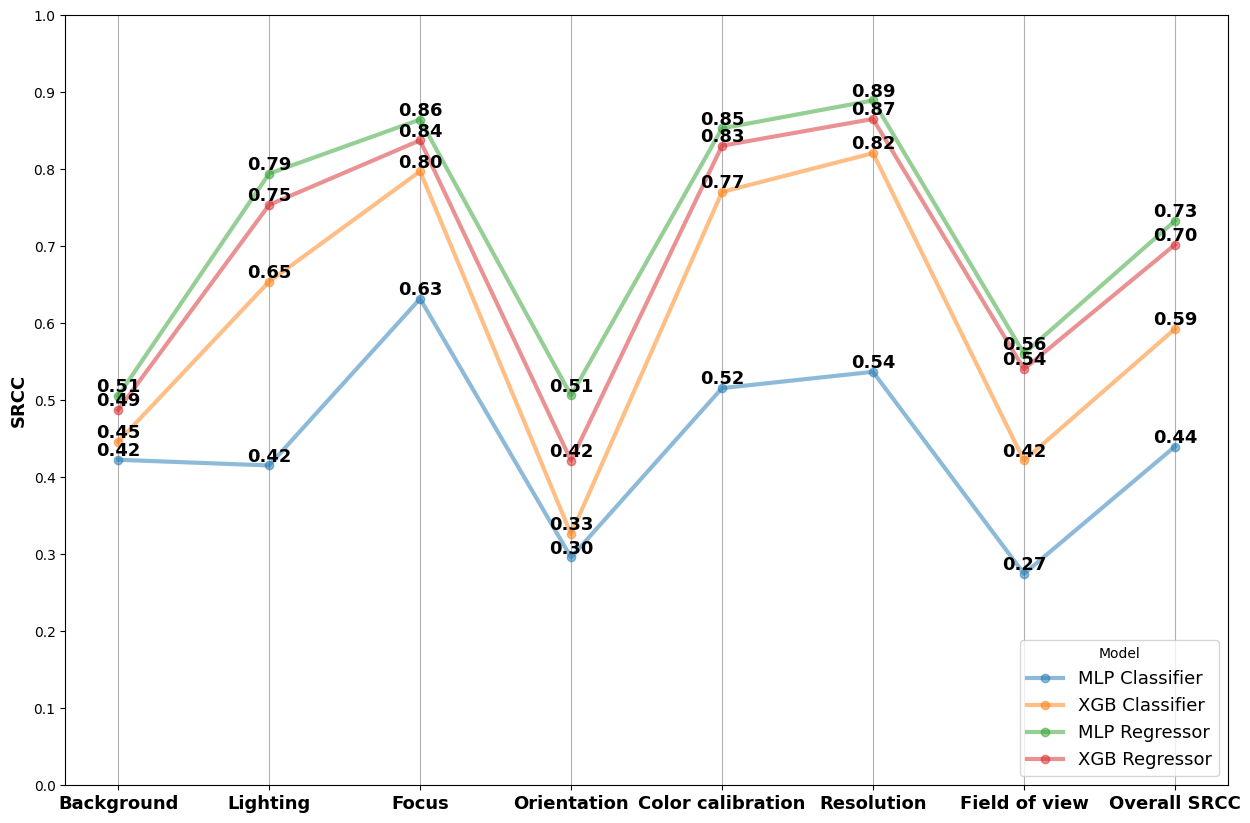
\includegraphics[keepaspectratio,width=12.5cm]{img/Model_SRCC.png}
    \caption{Parallel coordinate plot showing the best SRCC values for the four different models across the seven criteria and the overall SRCC. This plot highlights the performance of the MLP Regressor.}
    \label{fig:ModelSRCC}
\end{figure}
\clearpage
\subsection{Loss Curve Analysis}
\label{subsec:LossCurveAnalysis}
The loss curve in \autoref{fig:loss} shows the model's loss decreases over time for each distortion criterion during training. This visualization highlights the model’s performance improvement over time with each iteration. The maximum number of iterations was set to 500, and early stopping was enabled to prevent overfitting.
\begin{figure}[ht]
    \centering
    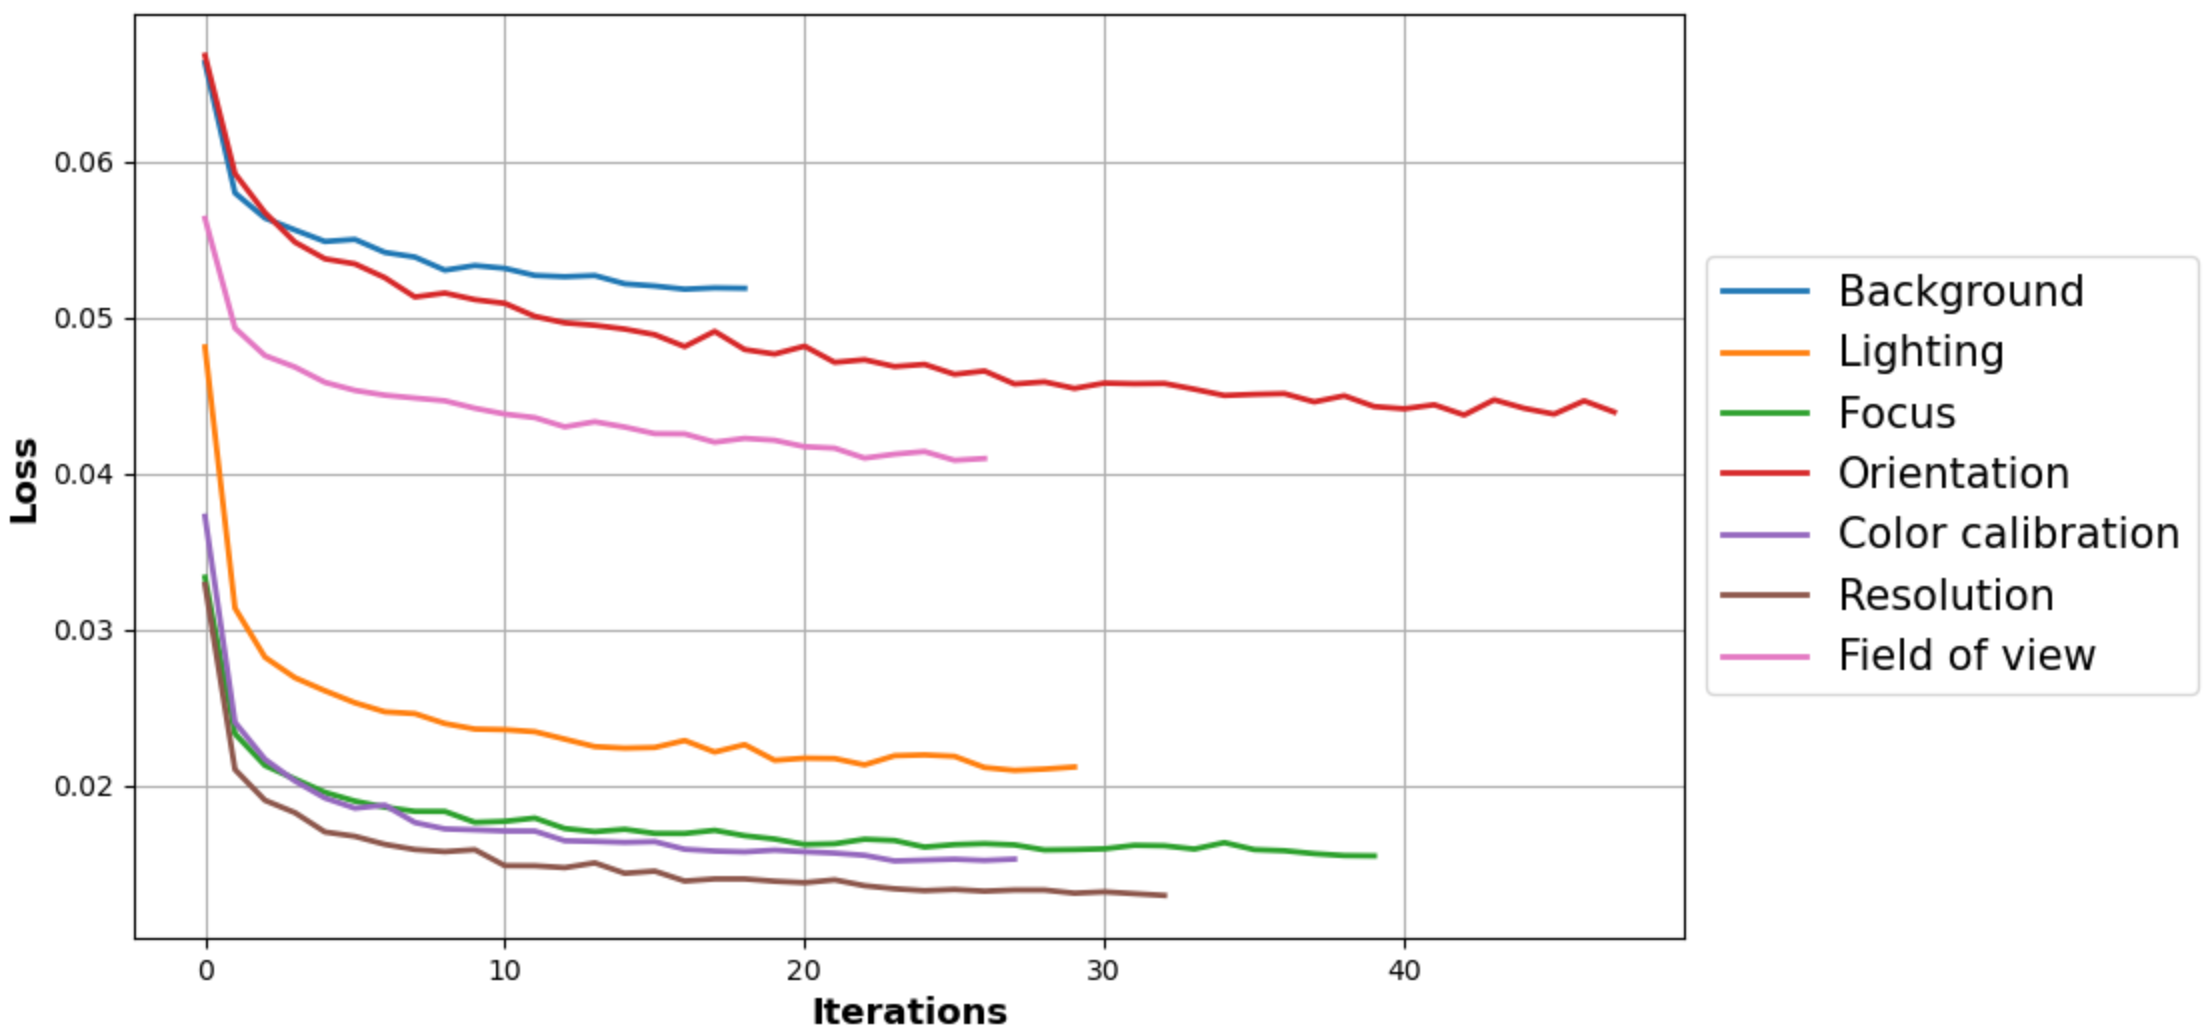
\includegraphics[keepaspectratio,width=15cm]{img/loss.png}
    \caption{Loss curve showing the reduction in loss for each distortion criterion during the training process. Each line represents a different criterion, showing how the model’s performance improves over time with each iteration.}
    \label{fig:loss}
\end{figure}
\subsection{Performance Metrics}
\label{subsec:PerformanceMetrics}
The performance of the final MLP regressor model on individual criteria is shown in \autoref{table:performance_metrics}. This table presents the performance metrics for the final MLP regressor model on 475 good quality Fitzpatrick images that were synthetically distorted. These metrics give a detailed view of the model’s strengths and weaknesses. \par
 \begin{table}[ht]
    \centering
    \begin{tabular}{|l|c|c|c|c|}
        \hline
        \textbf{Criteria} & \textbf{MAE} & \textbf{R\textsuperscript{2}} & \textbf{SRCC} & \textbf{Cohen's Kappa} \\
        \hline
        Background & 0.9684 & 0.2595 & 0.5422 & 0.4399 \\
        Lighting & 0.5726 & 0.6440 & 0.8028 & 0.7913 \\
        Focus & 0.4042 & 0.7385 & 0.8622 & 0.8568 \\
        Orientation & 0.9895 & 0.1824 & 0.4735 & 0.4102 \\
        Color calibration & 0.4905 & 0.7334 & 0.8622 & 0.8583 \\
        Resolution & 0.3642 & 0.7656 & 0.8722 & 0.8726 \\
        Field of view & 0.5474 & 0.5976 & 0.7710 & 0.7660 \\
        \hline
        \textbf{Overall} & \textbf{0.6195} & \textbf{0.5646} & \textbf{0.7507} & \textbf{0.7396} \\
        \hline
    \end{tabular}
    \caption{Performance Metrics for Each Distortion Criteria}
    \label{table:performance_metrics}
\end{table}

\clearpage
\subsection{Confusion Matrices}
\label{subsec:ConfusionMatrices}
In addition to numerical metrics, confusion matrices\footnote{from utils.visualization import plot\_all\_confusion\_matrices} were created for each criterion, as shown in \autoref{fig:confusion_matrices}. These matrices display where the model makes correct predictions and where it makes mistakes, showing a detailed view of its accuracy for each type of distortion. Furthermore, the confusion matrices also reveal any biases the model might have toward certain severity ranges, indicating whether it tends to predict only low or high severity levels, or if its predictions are skewed in some way. \par
\vspace{\baselineskip}
\begin{figure}[ht]
    \centering
    \begin{subfigure}[b]{0.32\textwidth}
        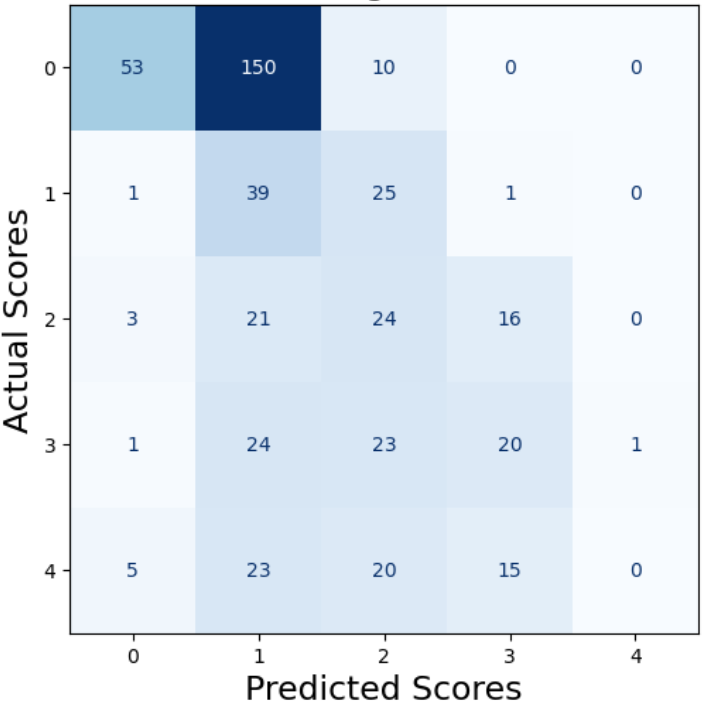
\includegraphics[width=\textwidth]{img/cm/bg.png}
        \caption{Background}
        \label{fig:cm_bg}
    \end{subfigure}
    \hfill
    \begin{subfigure}[b]{0.32\textwidth}
        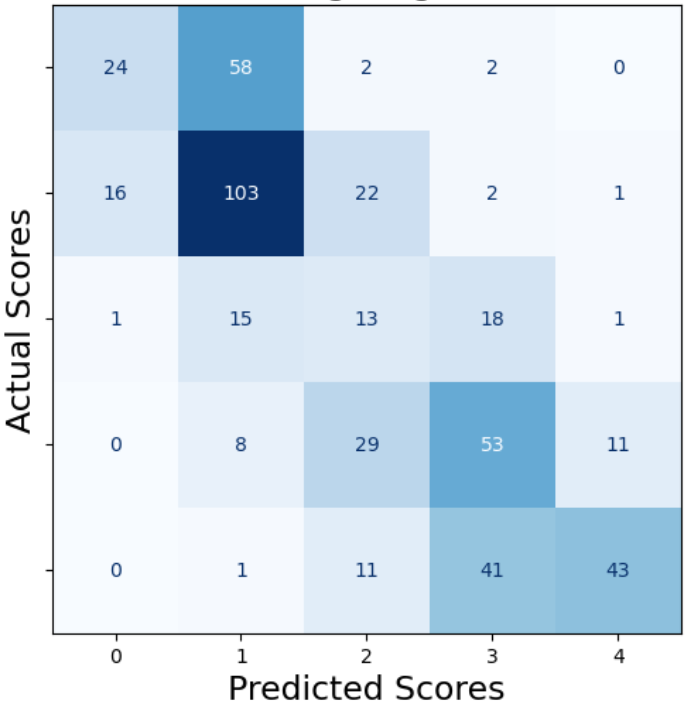
\includegraphics[width=\textwidth]{img/cm/light.png}
        \caption{Lighting}
        \label{fig:cm_light}
    \end{subfigure}
    \hfill
    \begin{subfigure}[b]{0.32\textwidth}
        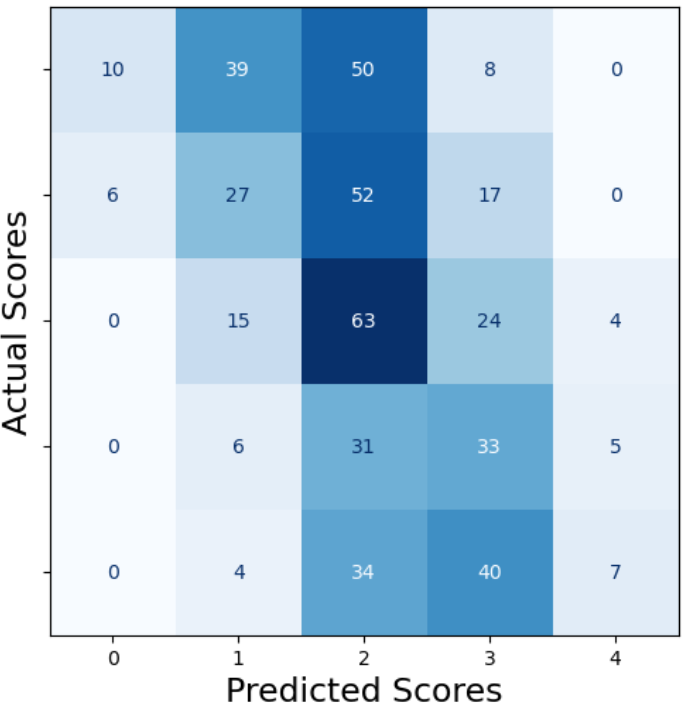
\includegraphics[width=\textwidth]{img/cm/orient.png}
        \caption{Orientation}
        \label{fig:cm_orient}
    \end{subfigure} 

    \begin{subfigure}[b]{0.24\textwidth}
        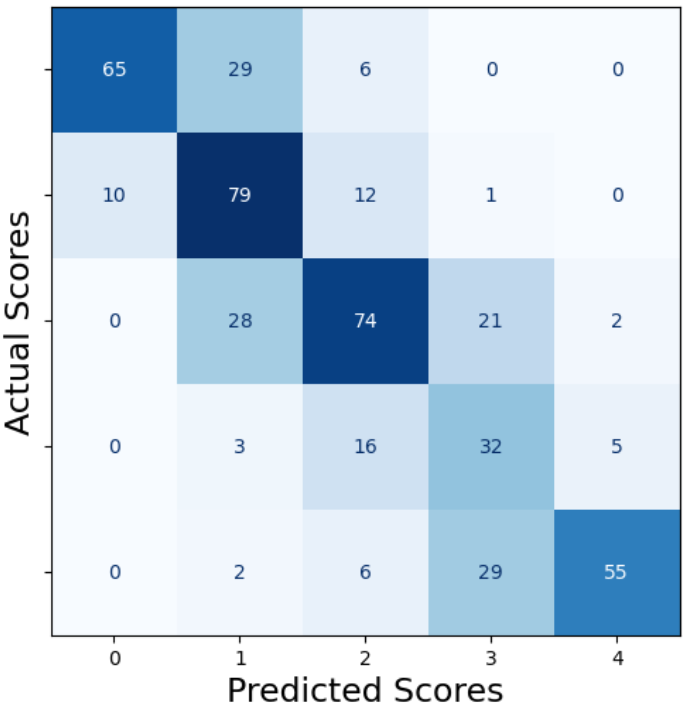
\includegraphics[width=\textwidth]{img/cm/foc.png}
        \caption{Focus}
        \label{fig:cm_foc}
    \end{subfigure}
    \hfill
    \begin{subfigure}[b]{0.24\textwidth}
        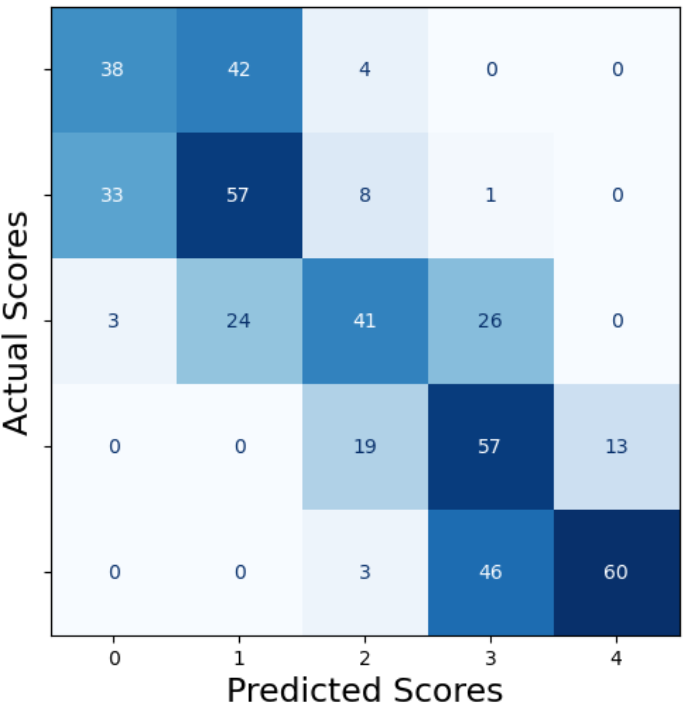
\includegraphics[width=\textwidth]{img/cm/cc.png}
        \caption{Color Calibration}
        \label{fig:cm_cc}
    \end{subfigure}
    \hfill
    \begin{subfigure}[b]{0.24\textwidth}
        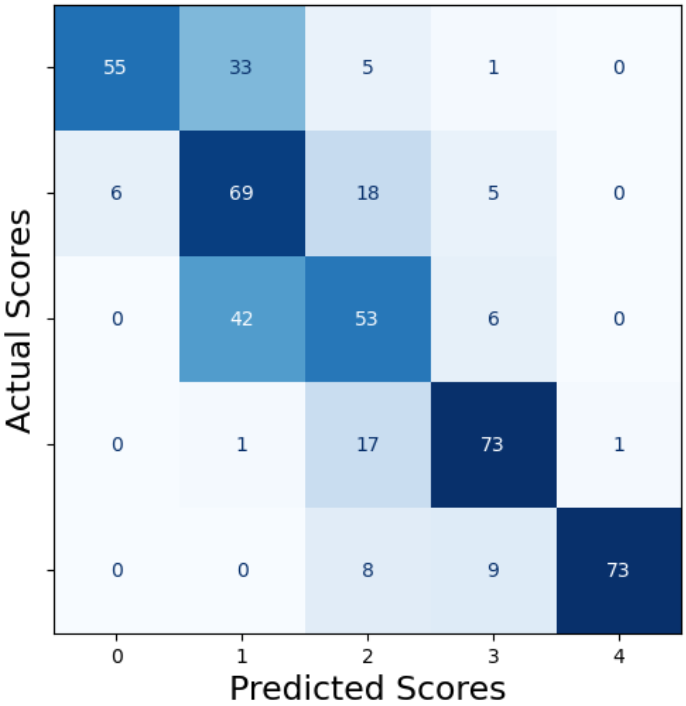
\includegraphics[width=\textwidth]{img/cm/res.png}
        \caption{Resolution}
        \label{fig:cm_res}
    \end{subfigure}
    \hfill
    \begin{subfigure}[b]{0.24\textwidth}
        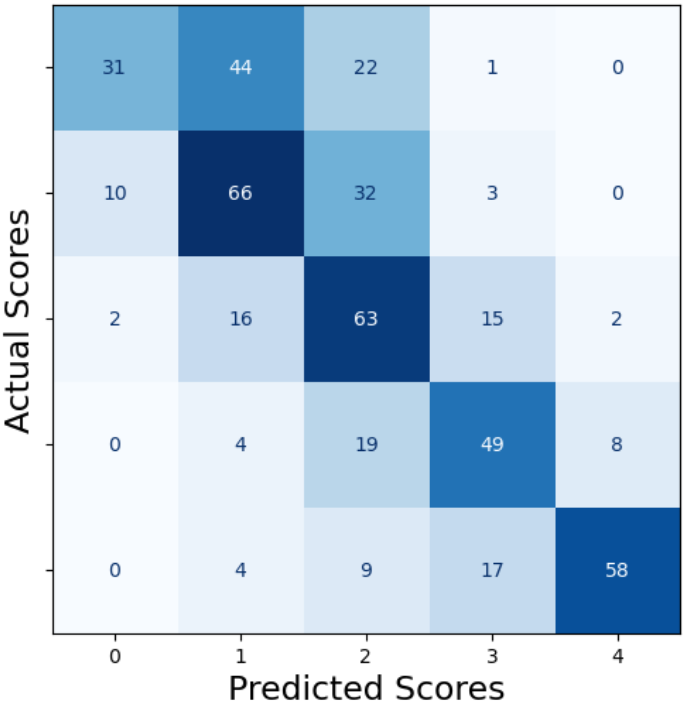
\includegraphics[width=\textwidth]{img/cm/fov.png}
        \caption{Field of View}
        \label{fig:cm_fov}
    \end{subfigure}
    \caption{Confusion matrices for the MLP Regressor model evaluated on the 475 images from the Fitzpatrick dataset. Each matrix corresponds to a specific distortion criterion and shows the actual scores on the y-axis and the predicted scores on the x-axis. Darker shades indicate higher counts, highlighting where the model's predictions match the actual values and where discrepancies occur.}
    \label{fig:confusion_matrices}
\end{figure}
\vspace{\baselineskip}
\noindent

\clearpage
\section{Model Predictions}
\label{sec:VisualizingPredictions}
To better understand the model’s performance on the two test sets (70 synthetic distorted images and 200 authentic images), radar charts\footnote{from utils.visualization import plot\_results} were created. These charts show the criteria on the outside, with severity ranges going from the center (0) to the outer edge (1), indicating high distortion for each criterion. These visualizations provide a clear and simple view of the model’s performance, showing its strengths and areas for improvement. \par
\subsection{Visualizations for Synthetic Distorted Images}
\label{subsec:SyntheticDistortedImages}
These visualizations, as shown in \autoref{fig:synthetic}, help to compare the model’s predictions with actual distortions for synthetic test images. This also helps to demonstrate the model’s accuracy in predicting various types of distortions. \par
\vspace{\baselineskip}
\noindent
The first column shows the original image, the second shows the distorted image, the third contains the actual labels, and the fourth presents the model’s predictions. \par
\begin{figure}[ht]
    \centering
    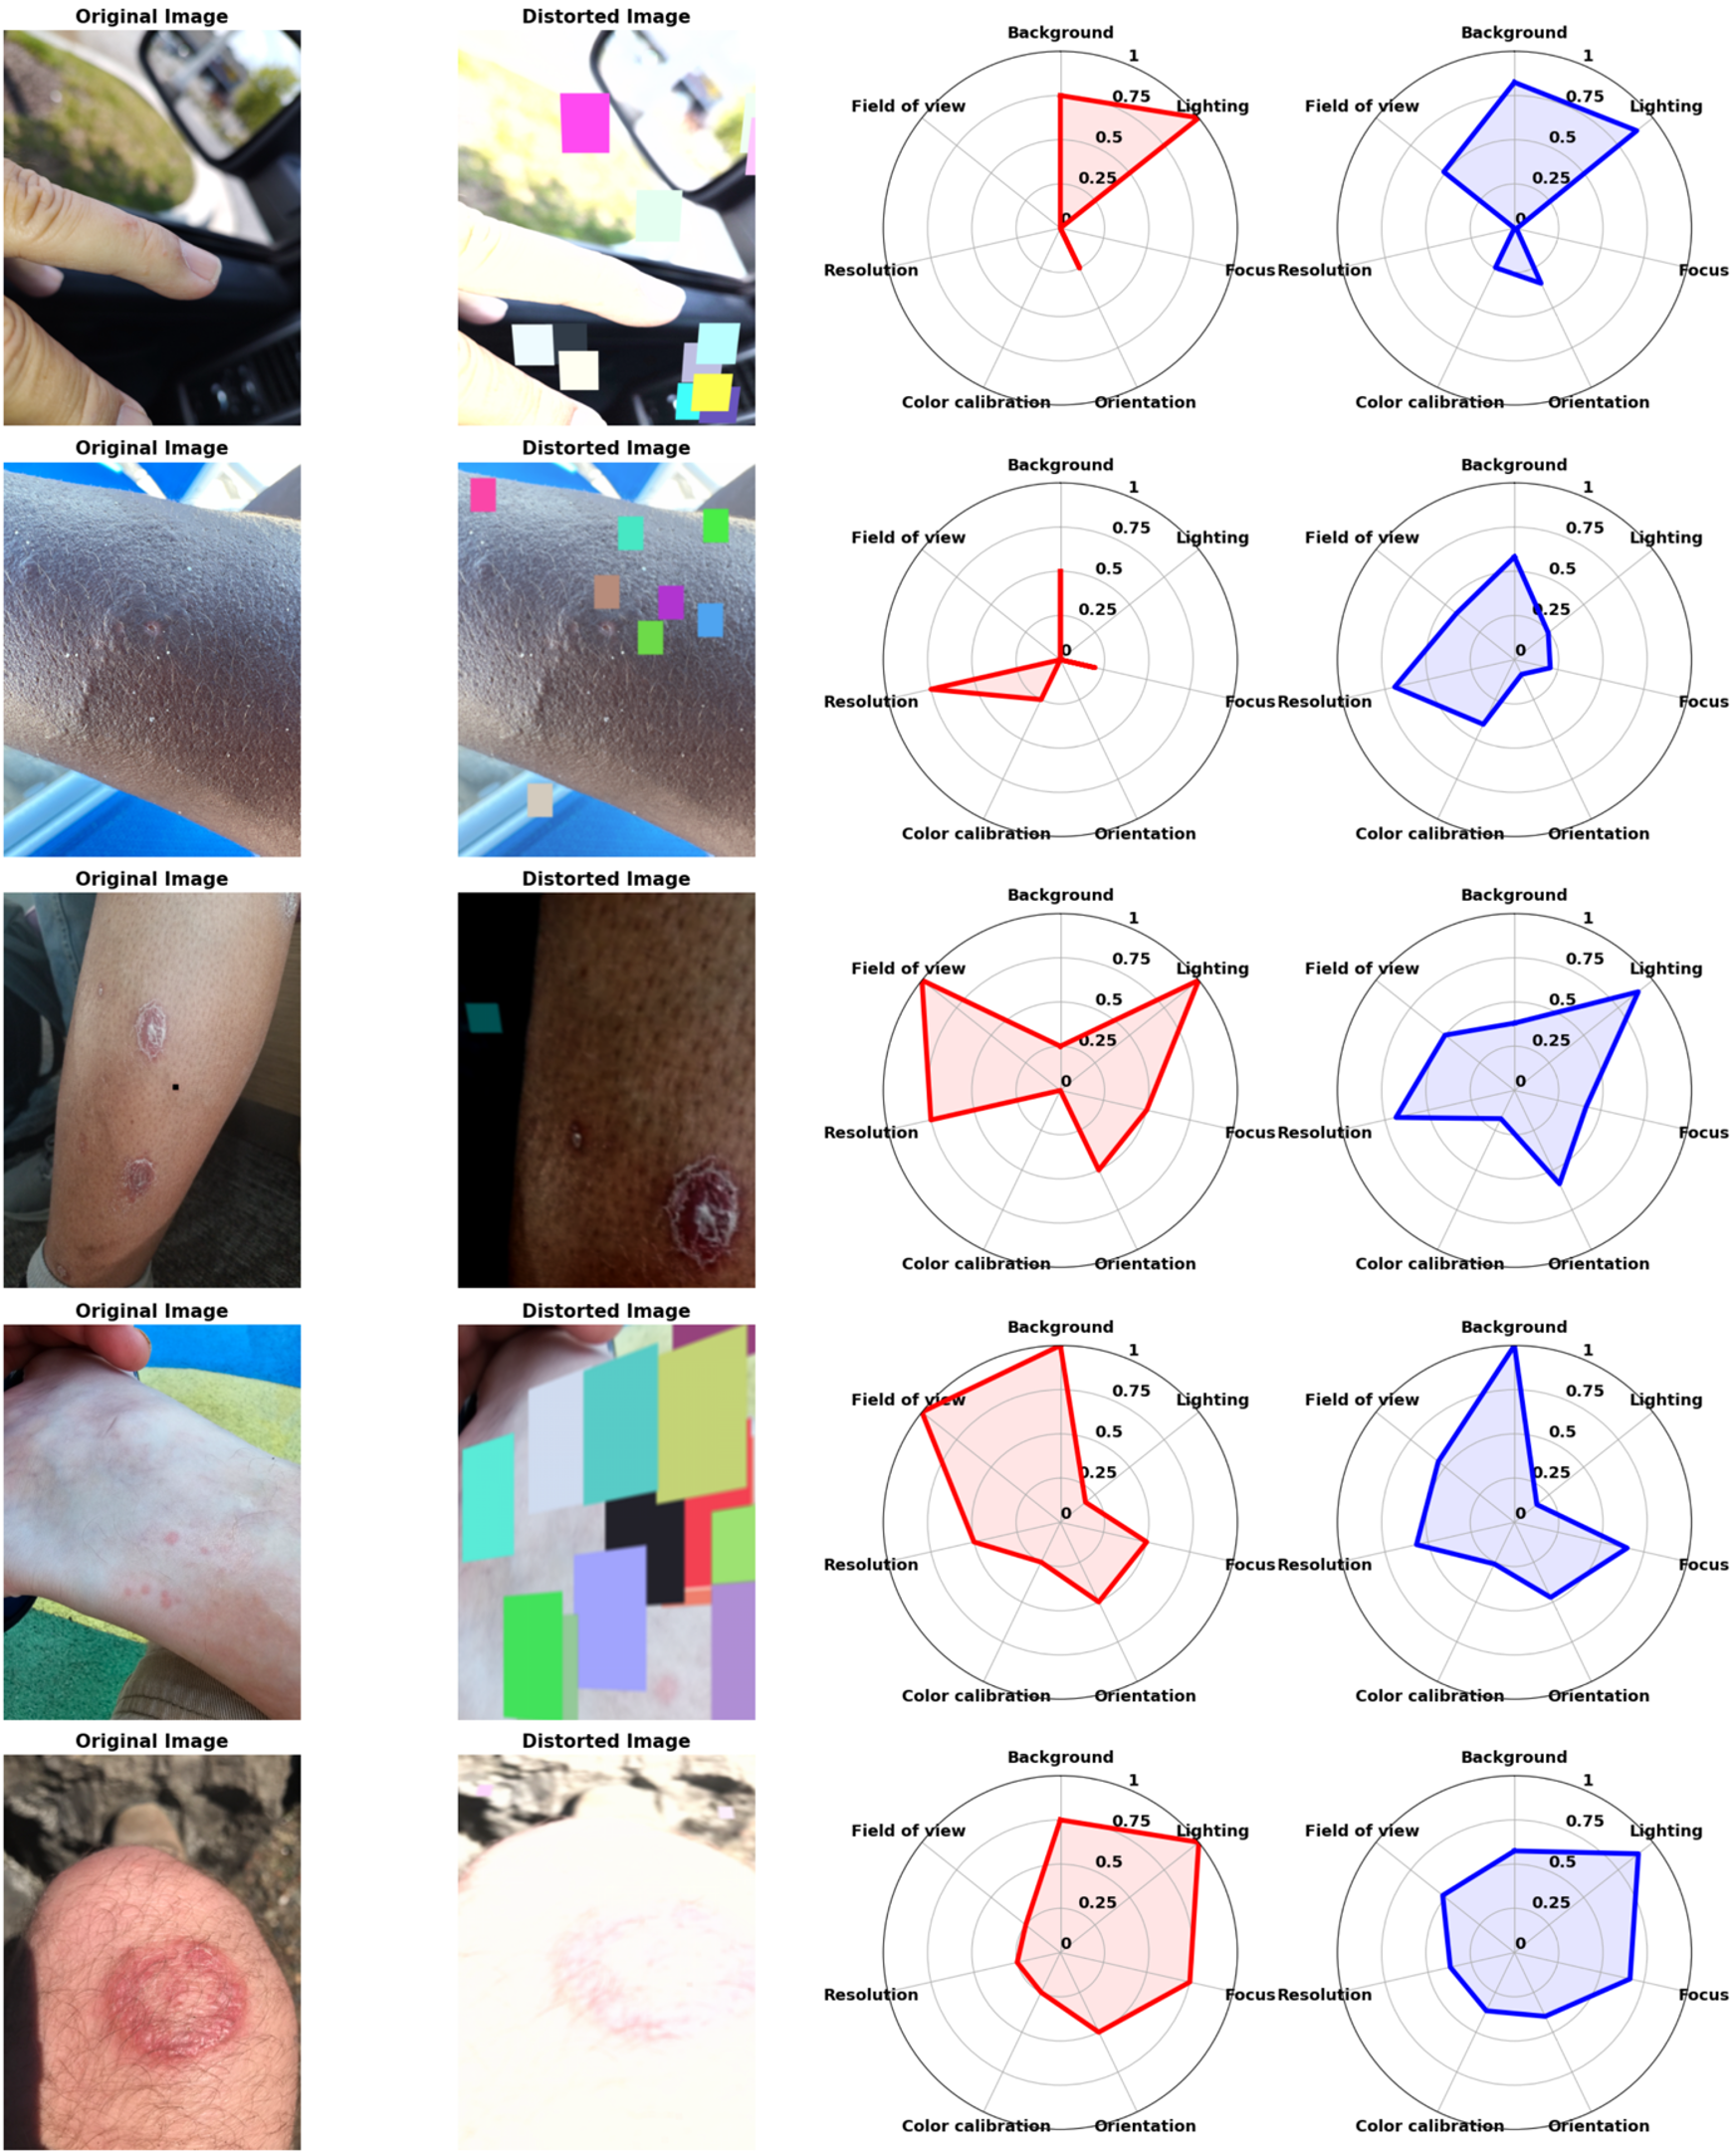
\includegraphics[keepaspectratio,width=15cm]{img/synthetic.png}
    \caption{Visualizations for the MLP Regressor model on 70 synthetic distorted images. The four-column layout shows the original image, the distorted image, the actual labels, and the model's predictions.}
    \label{fig:synthetic}
\end{figure}

\subsection{Visualizations for Authentic Images}
\label{subsec:AuthenticImages}
The visualizations, as shown in \autoref{fig:authentic}, compare the model's predictions with human-labeled scores for authentic images. This highlights the model's performance in real-world scenarios. \par
\vspace{\baselineskip}
\noindent
The first column shows the image, the second column displays the human-labeled scores, and the third column presents the model’s predictions. This comparison helps show how well the model’s predictions align with the human evaluations. \par
\begin{figure}[ht]
    \centering
    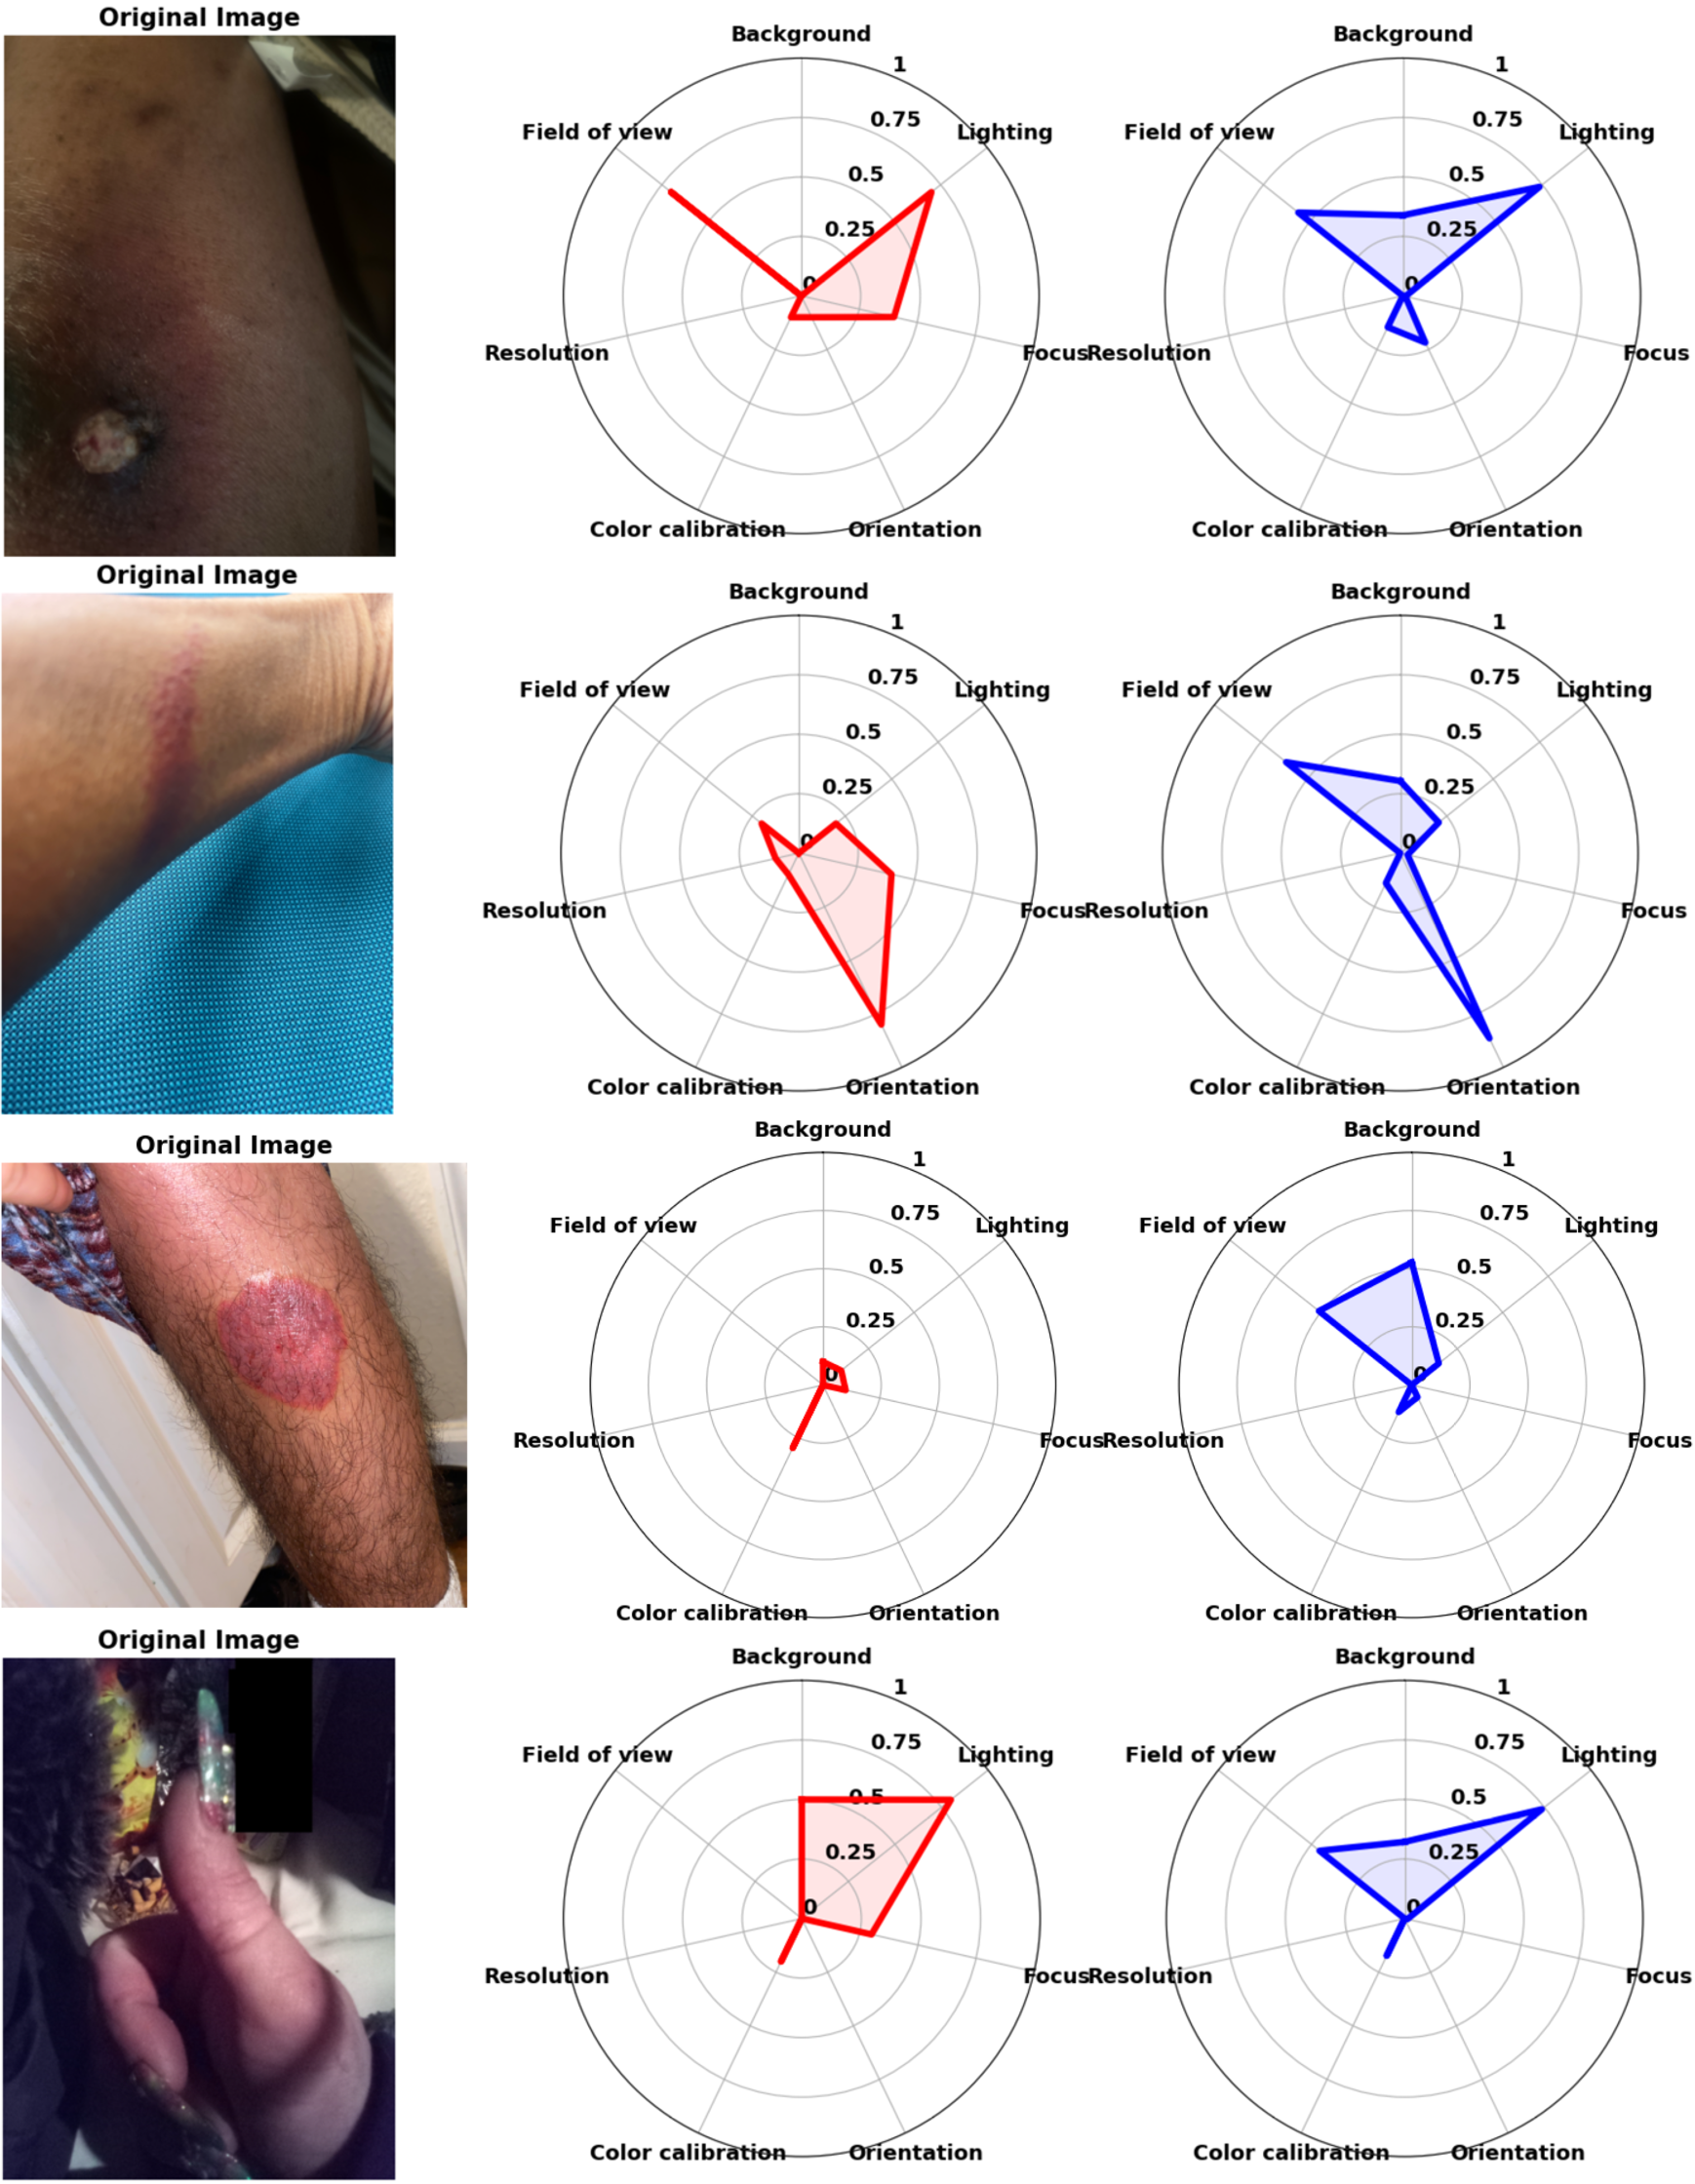
\includegraphics[keepaspectratio,width=15cm]{img/authentic.png}
    \caption{Visualizations for the MLP Regressor model on 200 authentic images. The three-column layout shows the image, the human-labeled scores, and the model's predictions.}
    \label{fig:authentic}
\end{figure}
\clearpage
\section{Assessing Training and Testing Images Quality}
\label{sec:TestingFilteredImages}
To verify the quality of the images used for training and see how they change after synthetic distortion, radar charts were created. These charts show the quality of the original training images and how they are affected by the distortions. Additionally, the quality of both the synthetic and authentic test images is assessed using the same method. These radar charts show a simple visual representation of the quality and the level of distortion across the seven criteria. \par
\subsection{Training Images Quality}
\label{subsec:TrainingImagesQuality}
\autoref{fig:SF} and \autoref{fig:FF} show the quality of the original SCIN and Fitzpatrick images, and the filtered good quality images, respectively. \autoref{fig:CF} shows the quality of the combined SCIN and Fitzpatrick images and the synthetically distorted images used for training the model. \par
\begin{figure}[ht]
    \centering
    \begin{subfigure}[b]{0.48\textwidth}
        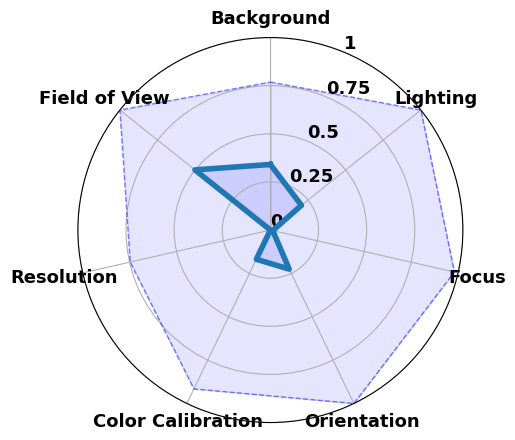
\includegraphics[width=\textwidth]{img/hept/SCIN10k.png}
        \caption{SCIN Images}
        \label{fig:SCIN10k}
    \end{subfigure}
    \hfill
    \begin{subfigure}[b]{0.48\textwidth}
        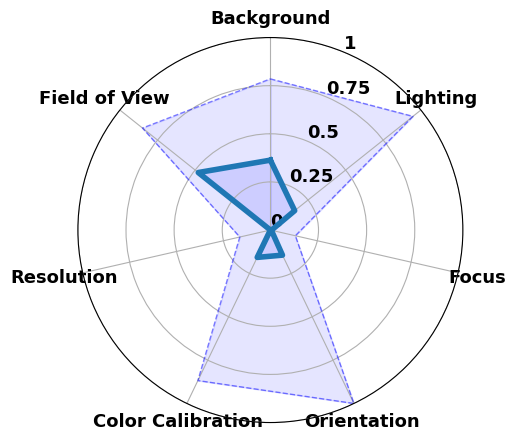
\includegraphics[width=\textwidth]{img/hept/SCIN.png}
        \caption{Filtered SCIN Images}
        \label{fig:SCIN}
    \end{subfigure}
    \hfill
    \caption{Radar charts for the SCIN dataset. (a) Original images from the SCIN dataset (10'379 images). (b) Filtered good quality images (475 images).}
    \label{fig:SF}
\end{figure}
\begin{figure}[ht]
    \centering
    \begin{subfigure}[b]{0.48\textwidth}
        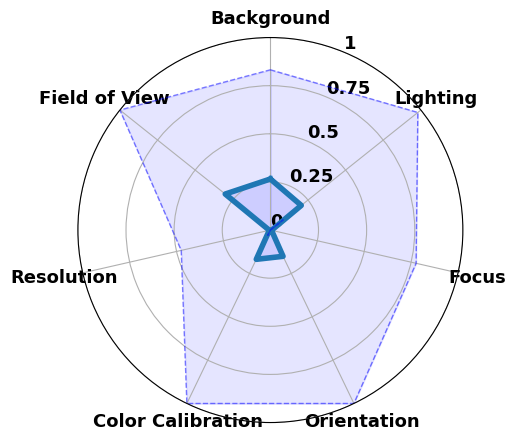
\includegraphics[width=\textwidth]{img/hept/Fitzpatrick17k.png}
        \caption{Fitzpatrick Images}
        \label{fig:Fitzpatrick17K}
    \end{subfigure}
    \hfill
    \begin{subfigure}[b]{0.48\textwidth}
        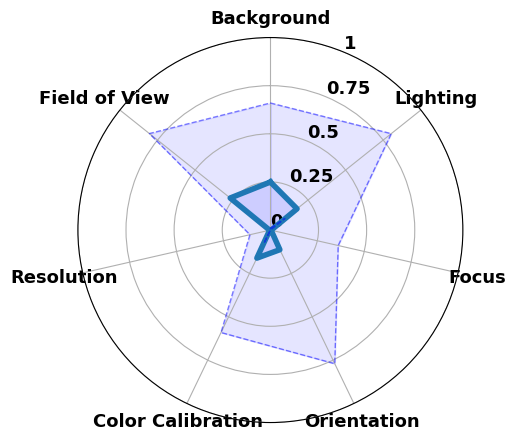
\includegraphics[width=\textwidth]{img/hept/F17K.png}
        \caption{Filtered Fitzpatrick Images}
        \label{fig:F17K}
    \end{subfigure}
    \hfill
    \caption{Radar charts for the Fitzpatrick dataset. (a) Original images from the Fitzpatrick dataset (16'577 images). (b) Filtered good quality images (475 images).}
    \label{fig:FF}
\end{figure}
\clearpage
\begin{figure}[ht]
    \centering
    \begin{subfigure}[b]{0.48\textwidth}
        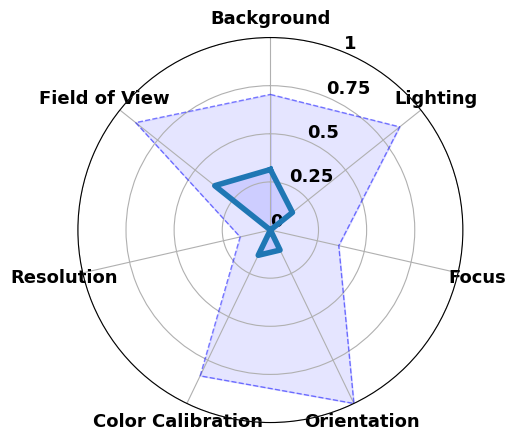
\includegraphics[width=\textwidth]{img/hept/combined.png}
        \caption{Combined SCIN and Fitzpatrick Images}
        \label{fig:combined}
    \end{subfigure}
    \hfill
    \begin{subfigure}[b]{0.48\textwidth}
        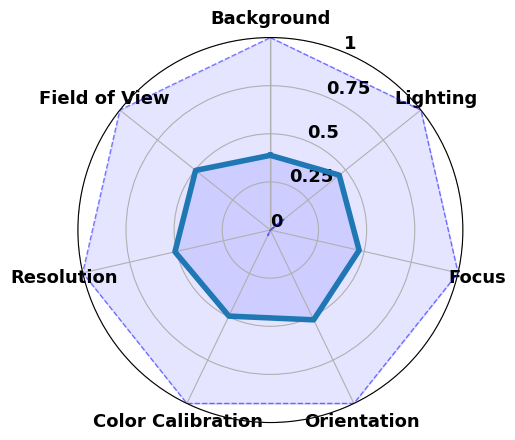
\includegraphics[width=\textwidth]{img/hept/comb_synthetic.png}
        \caption{Synthetically Distorted Images}
        \label{fig:comb_synthetic}
    \end{subfigure}
    \hfill
    \caption{Combined dataset analysis. (a) Combined SCIN and Fitzpatrick images (950 images). (b) Synthetically distorted images.}
    \label{fig:CF}
\end{figure}
\clearpage
\subsection{Test Images Quality}
\label{subsec:TestImagesQuality}
\autoref{fig:T1} shows the quality of the filtered good quality test images and the synthetically distorted test images. \autoref{fig:T2} shows the quality of the authentic test images from the SCIN dataset. These radar charts provide a visual representation of the quality of the test images and the level of distortion across the seven criteria. \par
\begin{figure}[ht]
    \centering
    \begin{subfigure}[b]{0.48\textwidth}
        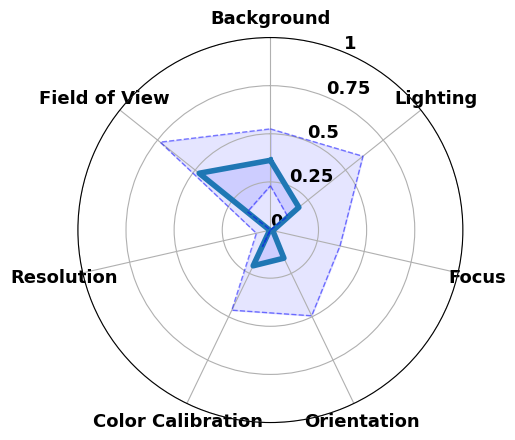
\includegraphics[width=\textwidth]{img/hept/test_70.png}
        \caption{Filtered Test Images}
        \label{fig:test_70}
    \end{subfigure}
    \hfill
    \begin{subfigure}[b]{0.48\textwidth}
        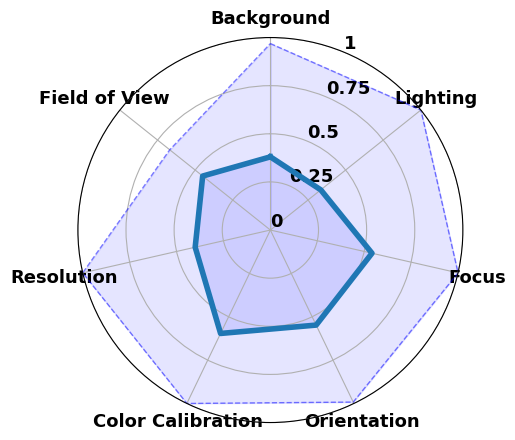
\includegraphics[width=\textwidth]{img/hept/test_70_synthetic.png}
        \caption{Synthetically Distorted Test Images}
        \label{fig:test_70_synthetic}
    \end{subfigure}
    \hfill
    \caption{Synthetic test set analysis. (a) Filtered good quality test images (70 images, independent of training set). (b) Synthetically distorted test images.}
    \label{fig:T1}
\end{figure}

\begin{figure}[ht]
    \centering
    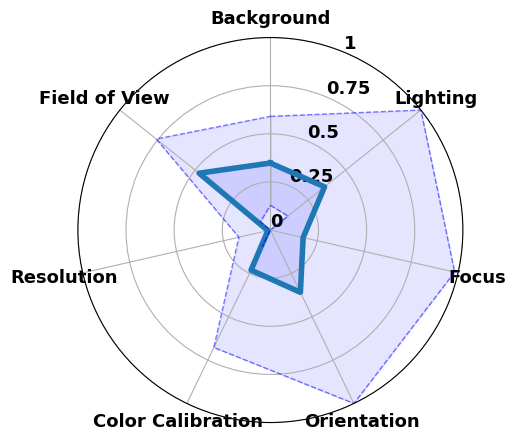
\includegraphics[keepaspectratio,width=7cm]{img/hept/test_200.png}
    \caption{Authentic test set from the SCIN dataset, independent of the training images, showing real-world distortions.}
    \label{fig:T2}
\end{figure}
\clearpage
\section{Comparison with ARNIQA Predictions}
\label{sec:ComparisonARNIQA}
This section compares the model’s predictions with the predictions from ARNIQA for both synthetic and authentic test sets, highlighting how well the model aligns with established quality scores. \par
\begin{figure}[ht]
    \centering
    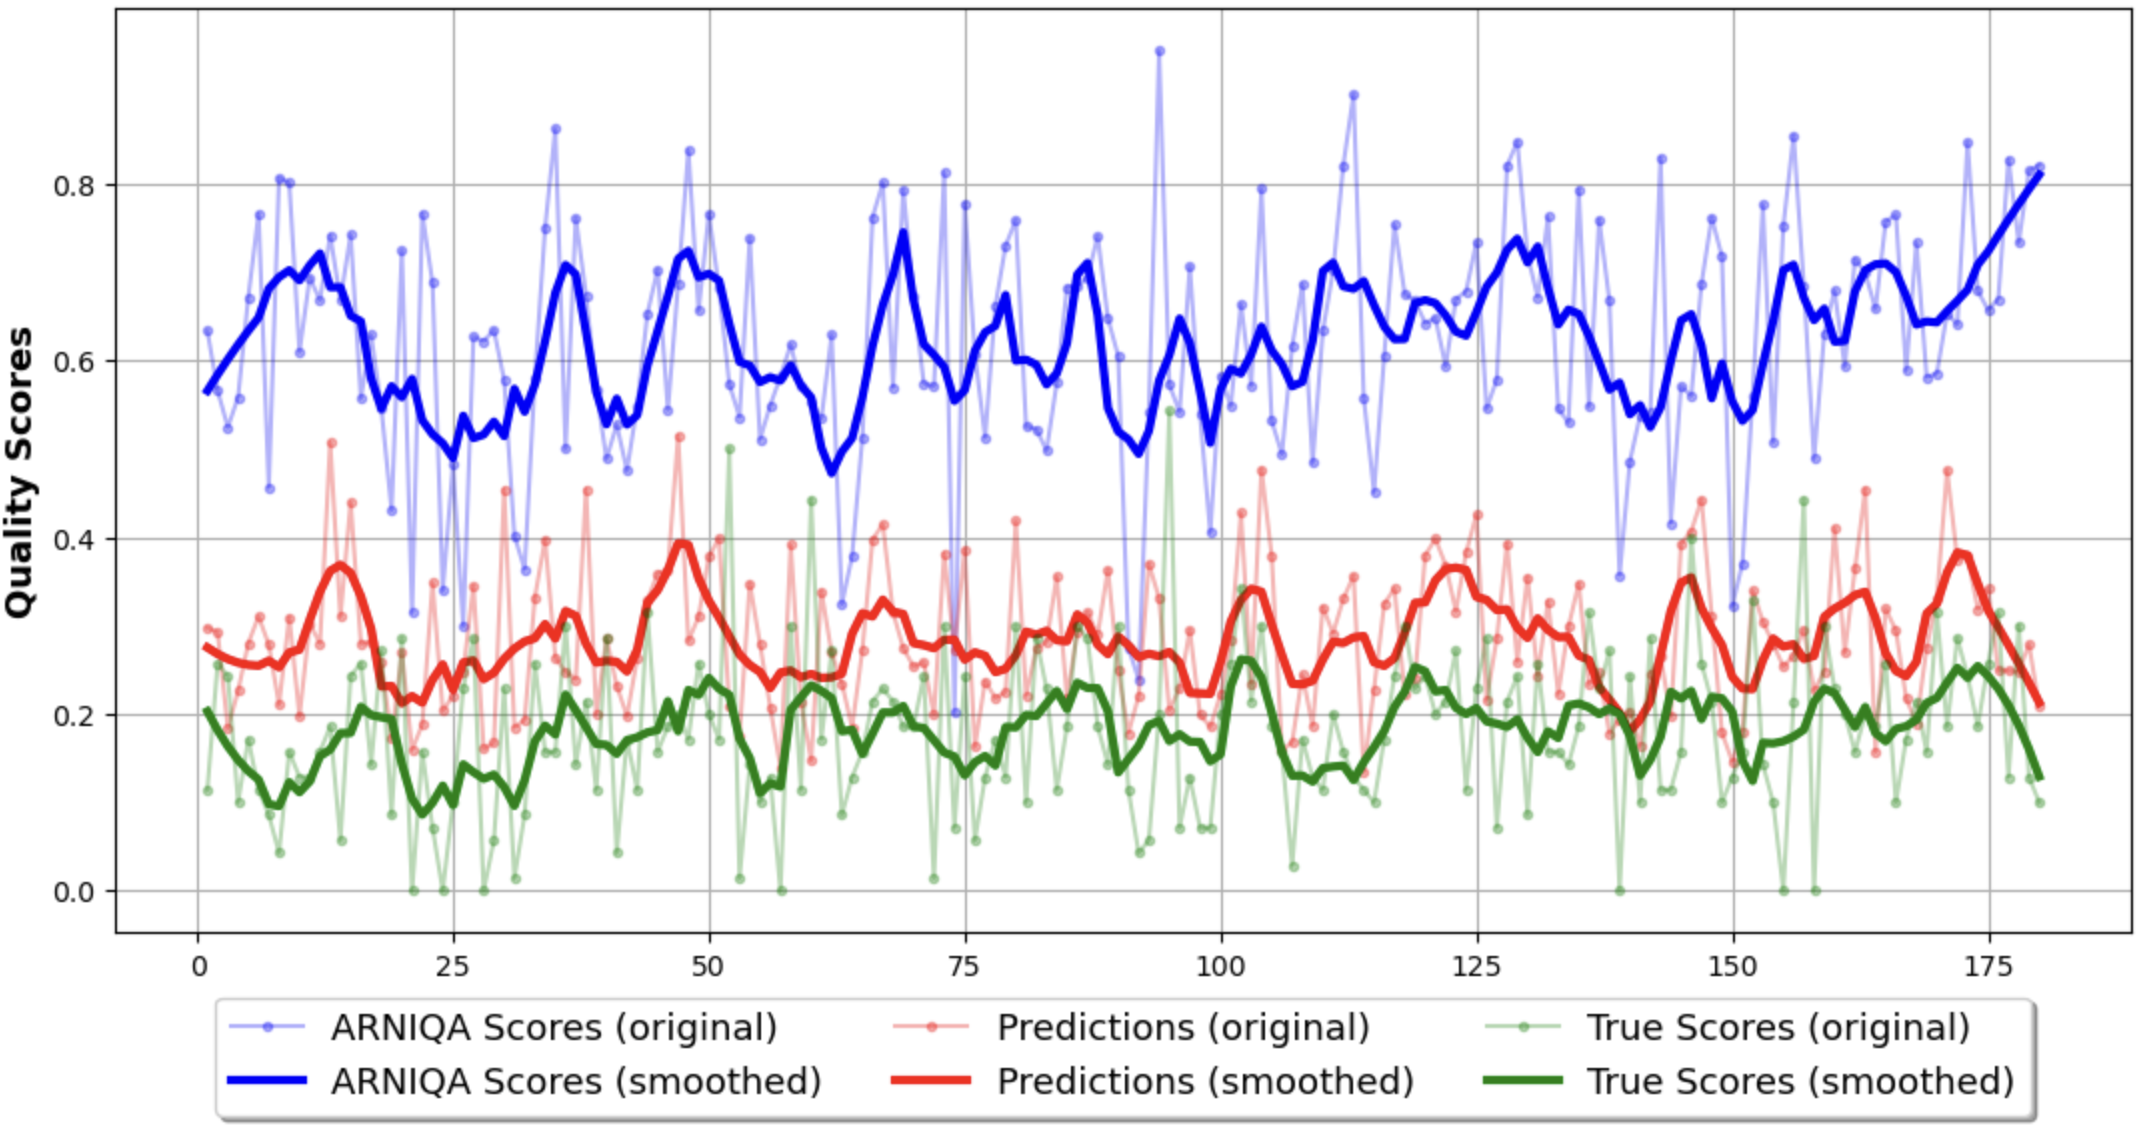
\includegraphics[keepaspectratio,width=13cm]{img/hept/test_200_arniqa.png}
    \caption{Comparison of ARNIQA Scores, Model Predictions, and True Scores for 200 authentic images from the SCIN Dataset. This plot presents the quality scores for each image, showcasing how well the model’s predictions align with the ARNIQA scores and the true scores.}
    \label{fig:T2A}
\end{figure}

\begin{figure}[ht]
    \centering
    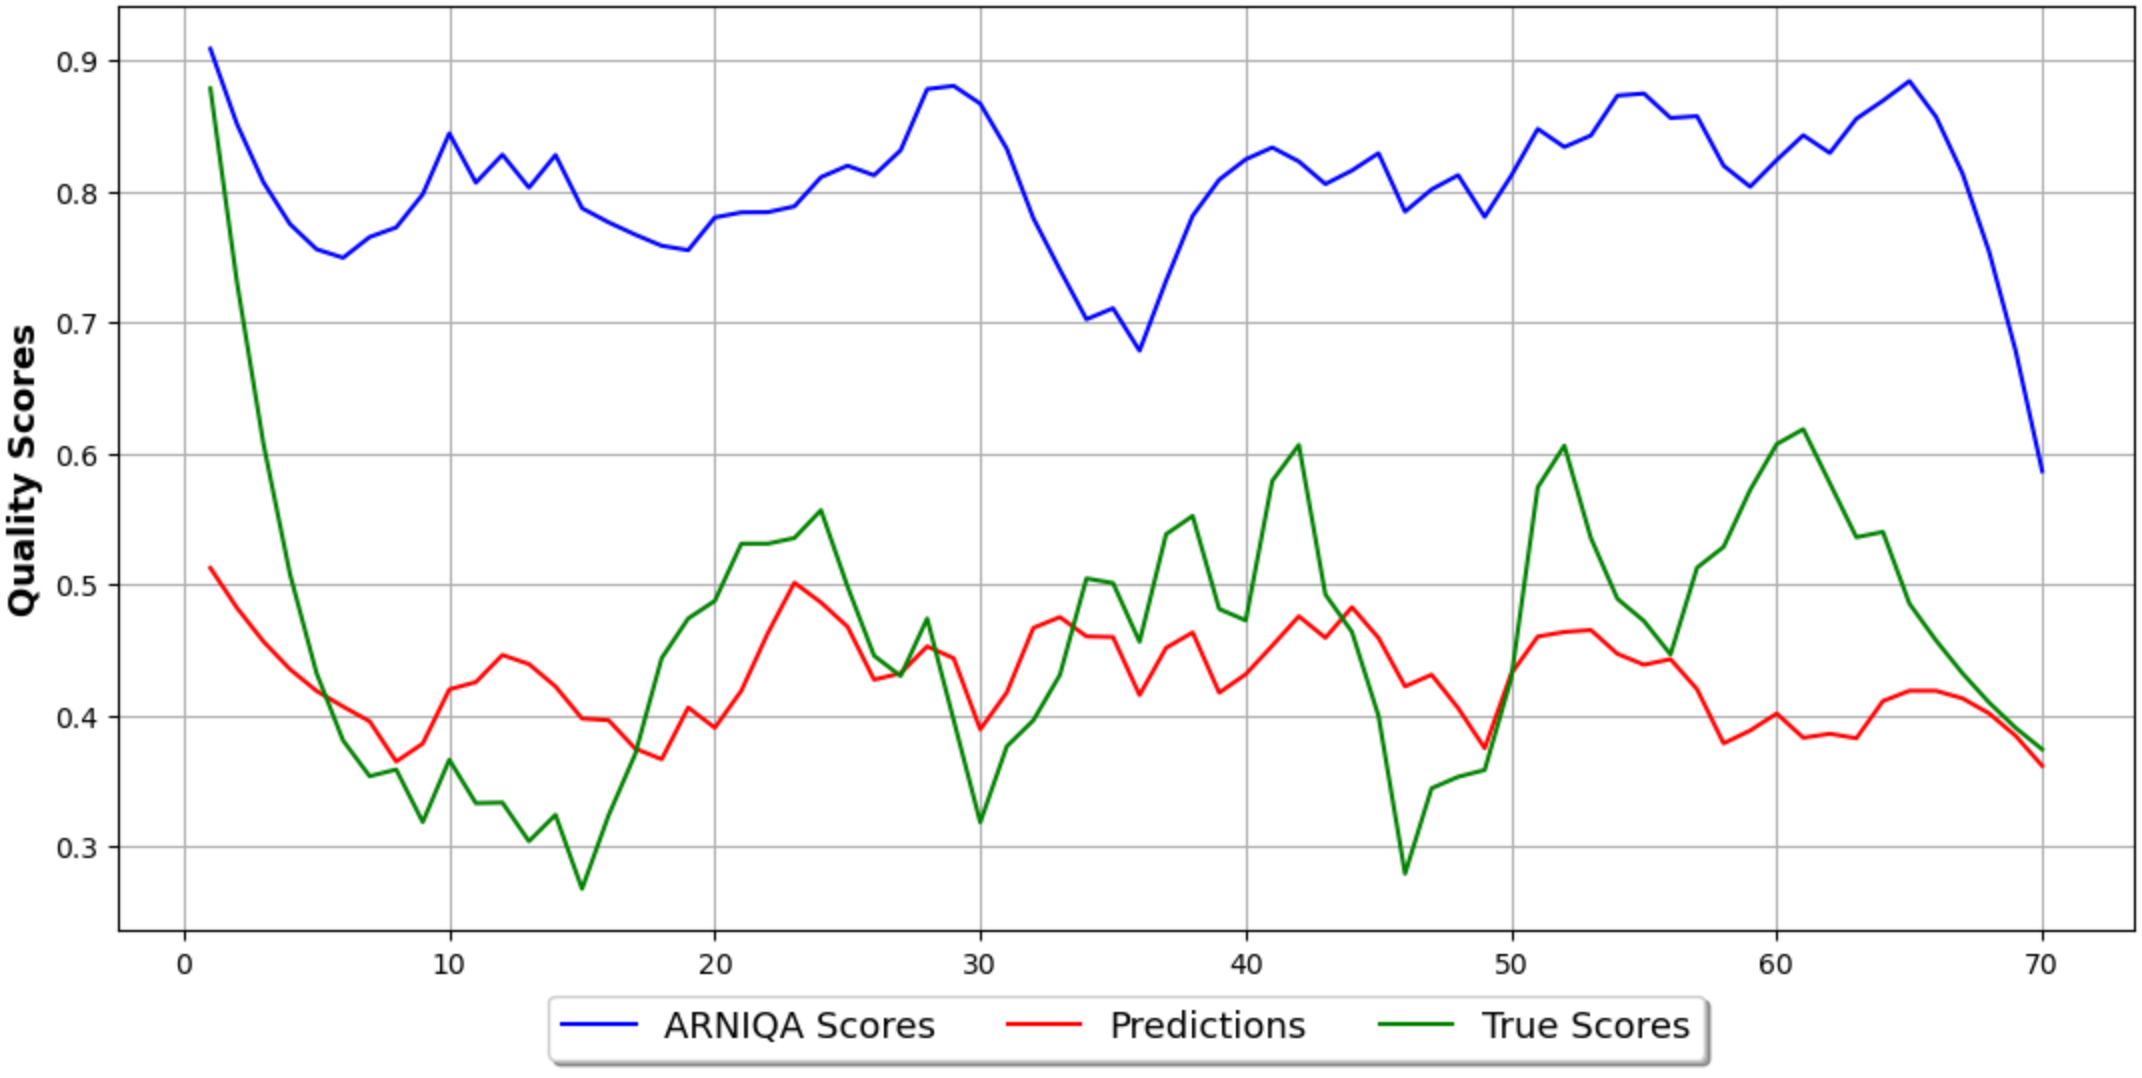
\includegraphics[keepaspectratio,width=13cm]{img/hept/test_70_arniqa.png}
    \caption{Comparison of ARNIQA Scores, Model Predictions, and True Scores for 70 synthetically distorted images from the SCIN dataset. This plot shows the quality scores for each image, highlighting the performance of the model against ARNIQA’s predictions and the actual scores.}
    \label{fig:T7A}
\end{figure}